\documentclass[10pt,fleqn]{article}
\usepackage{hyperref}
\usepackage{graphicx}


\setlength{\topmargin}{-.75in}
\addtolength{\textheight}{2.00in}
\setlength{\oddsidemargin}{.00in}
\addtolength{\textwidth}{.75in}

\nofiles

\pagestyle{empty}

\setlength{\parindent}{0in}

% new math commands


\setlength{\oddsidemargin}{-0.25in}
\setlength{\evensidemargin}{-0.25in}
\setlength{\textwidth}{6.75in}
\setlength{\headheight}{0.0in}
\setlength{\topmargin}{-0.25in}
\setlength{\textheight}{9.00in}

\makeindex

\usepackage{mathrsfs}

%\usepackage[pdftex]{graphicx}
\usepackage{epstopdf}

\newcounter{beans}

\newcommand{\ds}{\displaystyle}
\newcommand{\limit}[2]{\displaystyle\lim_{#1\to#2}}

\newcommand{\binomial}[2]{\ \left( \begin{array}{c}
                                  #1 \\
                                  #2
                                 \end{array}
                            \right) \
                         }
\newcommand{\ExampleRule}[2]
  {
  \noindent
  \rule{\linewidth}{1pt}
  \begin{example}
    #1
    \label{#2}
  \end{example}
  \rule{\linewidth}{1pt}
  \vskip0.125in
  }

\newcommand{\defbox}[1]
  {
   \ \\
   \noindent
   \setlength\fboxrule{1pt}
   \fbox{
        \begin{minipage}{6.5in}
          #1
        \end{minipage}
        }
   \ \\
  }
\newcommand{\verysmallworkbox}[1]
  {
   \ \\
   \noindent
   \setlength\fboxrule{1pt}
   \fbox{
        \begin{minipage}{6.5in}
           #1
           \ \\
           \vskip0.5in \ \\
           \ \\
        \end{minipage}
        }
   \ \\
  }
\newcommand{\smallworkbox}[1]
  {
   \ \\
   \noindent
   \setlength\fboxrule{1pt}
   \fbox{
        \begin{minipage}{6.5in}
           #1
           \ \\
           \vskip2.5in \ \\
           \ \\
        \end{minipage}
        }
   \ \\
  }
\newcommand{\halfworkbox}[1]
  {
   \ \\
   \noindent
   \setlength\fboxrule{1pt}
   \fbox{
        \begin{minipage}{6.5in}
           #1 \hfill
           \ \\
           \vskip3.25in \ \\
           \ \\
        \end{minipage}
        }
   \ \\
  }
\newcommand{\largeworkbox}[1]
  {
   \ \\
   \noindent
   \setlength\fboxrule{1pt}
   \fbox{
        \begin{minipage}{6.5in}
           #1
           \ \\
           \vskip7.5in \ \\
           \ \\
        \end{minipage}
        }
   \ \\
  }
\newcommand{\flexworkbox}[2]
  {
   \ \\
   \noindent
   \setlength\fboxrule{1pt}
   \fbox{
        \begin{minipage}{6.5in}
           #1
           \ \\

           \vskip#2 \ \\
           \ \\
        \end{minipage}
        }
   \ \\
  }


% symbols for sets of numbers

\newcommand{\natnumb}{$\cal N$}
\newcommand{\whonumb}{$\cal W$}
\newcommand{\intnumb}{$\cal Z$}
\newcommand{\ratnumb}{$\cal Q$}
\newcommand{\irrnumb}{$\cal I$}
\newcommand{\realnumb}{$\cal R$}
\newcommand{\cmplxnumb}{$\cal C$}

% misc. commands

\newcommand{\mma}{{\it Mathematica}}
\newcommand{\sech}{\mbox{ sech}}
 
\newtheorem{theorem}{Theorem}
\newtheorem{example}{Example}
\newtheorem{definition}{Definition}
\newtheorem{problem}{Problem}

\setcounter{secnumdepth}{2}
\setcounter{tocdepth}{4}


\begin{document}
%%%%%%%%%%%%%%%%%%%%%%%%%%%%%%%%%%%%%%%%%%%%%%%%%%%%%%%%%%%%%%%%%%%%%%%%%%%%%%%%
%%%%%%%%%%%%%%%%%%%%%%%%%%%%%%%%%%%%%%%%%%%%%%%%%%%%%%%%%%%%%%%%%%%%%%%%%%%%%%%%
\vskip0.1in\hrule\vskip0.1in
\noindent
{\bf Math 4610 Fundamentals of Computational Mathematics  - Topic 5.}
\vskip0.1in\hrule\vskip0.1in

This topic covers information on how to work once a terminal is up and running
on your computer. A Linux/Unix operating system should be running in the
terminal. In most real computational settings, it is important to be able to
work using a command line to create files, modify these files, compile
code, and a number of other tasks. You can invoke multiple terminals and work on
multiple files at the same time. Your instructor has three or four terminals
open at any given time. One to edit files, one to compile and execute code, and
the third to display results. The homework and projects assigned in the class
will typically require the use of a terminal to complete the work.

We will eventually use High Performance Computing (HPC) resources at the Center
for High Performance Computing (CHPC) at the University of Utah to work on a
project or two. The access we will have will be through the terminals or
terminal emulators running Linux/Unix operating systems. So, it is important to
be familiar with at least a few basic Linux/Unix commands. In this section of
the notes we will work through a few of the more important commands needed. We
will also introduce more commands with options as we work through the semester.

In general, a Linux/Unix command can be written in the form:
\begin{verbatim}

   % command [options] [input parameters]

\end{verbatim}
where the \% is the prompt for entering a command and \lq\lq command\rq\rq\ is
replaced with the command. For example, replacing \lq\lq command\rq\rq with
the string \lq\lq pwd\rq\rq gives
\begin{verbatim}

   % pwd 

\end{verbatim}
The options and parameters in the general form may or may not be needed
depending on what you are trying to do. Note that the pwd command will display
the (p)resent (w)orking (d)irectory. In most cases, the pwd command will not
need any options or parameters. When we compile code, it is common to use a
number of options on the compiler commands.

Each of the subsections below will cover a single command to help you get
started. There are hundreds of commands that can be used from within a terminal.
Some of these commands can be unforgiving - there is not trash folder that will
save you from accidently removing a file. Note that there are some safety
measures that one can add. See the file remove command (rm) below.

Another important issue that any computational person should be aware of is that
there are a number of shells that you can work in. A command shell, say bash,
will have a slightly different flavor of commands and syntac. The shells that
most use are bash, csh, tcsh, and ksh. It is probably best to select a shell,
like bash or tcsh, and stick with that throughout the semester. Finally, a good
computational person is able to chain together a set of commands to perform a
sequence of commands. This sometimes referred to as shell programming. It is an
incredibly useful skill to have. However, shell programming is beyond the scope
of this course - meaning we can get by without it.
%%%%%%%%%%%%%%%%%%%%%%%%%%%%%%%%%%%%%%%%%%%%%%%%%%%%%%%%%%%%%%%%%%%%%%%%%%%%%%%%
%%%%%%%%%%%%%%%%%%%%%%%%%%%%%%%%%%%%%%%%%%%%%%%%%%%%%%%%%%%%%%%%%%%%%%%%%%%%%%%%
\vskip0.1in\hrule\vskip0.1in
\noindent
{\large{\bf
Linux Commands for Math 4610 at USU:} List the Contents of the Home Folder}
\vskip0.1in\hrule\vskip0.1in
\noindent
Once a terminal is running, the first thing we probably want to do is to look at
what is in a the directory we are in. It is important to know where you are at
in a directory tree and the like. This also serves as a first linux or unix
command. In the screenshot below there are a couple of versions of a command
that will list files and folders with more or less information. Note that most
linux commands look like the general command form given above.
\vskip0.1in\hrule\vskip0.1in
\vfill
\begin{figure}[h]
\centering
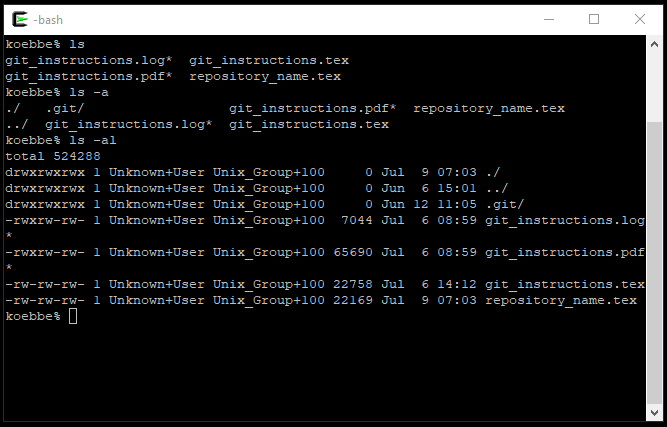
\includegraphics{../images/cygwin_02.png}
\caption{Two versions of the ls command used to list the contents of the curtent
         directory. Screenshot taken using {\bf Snip \& Sketch}. This is an app
         on my Windows 10 box}
\end{figure}
\eject
%%%%%%%%%%%%%%%%%%%%%%%%%%%%%%%%%%%%%%%%%%%%%%%%%%%%%%%%%%%%%%%%%%%%%%%%%%%%%%%%
%%%%%%%%%%%%%%%%%%%%%%%%%%%%%%%%%%%%%%%%%%%%%%%%%%%%%%%%%%%%%%%%%%%%%%%%%%%%%%%%
\vskip0.1in\hrule\vskip0.1in
\noindent
{{\bf
Cygwin Primer for Math 4610 at USU:} Directory Commands} 
\vskip0.1in\hrule\vskip0.1in
\noindent
You will need to create files and folders, move files and folders, remove files,
and perform other operations to directories to keep work organized. The
{\bf mkdir} command allows a persion to create a new directory in the current
working directory. This is the same thing tha Windows Explorer allows you to do
with a popup menu (New Folder). There will be many places where a directory
structure will be required. You can remove a directory with the
{\bf rmdir} command. The {\bf cd} command can be used to navigate through a
directory structure. Finally, on this screen capture, the {\bf pwd} command is
used to determine the current working directory. This can be used to figure out
where you are in a directory structure.
\begin{verbatim}

    % pwd                 current working directory
    % cd                  change working directory
    % mkdir               make a new directory
    % rmdir               remove an existing directory

\end{verbatim}
\vskip0.1in\hrule\vskip0.1in
\vfill
\begin{figure}[h]
\centering
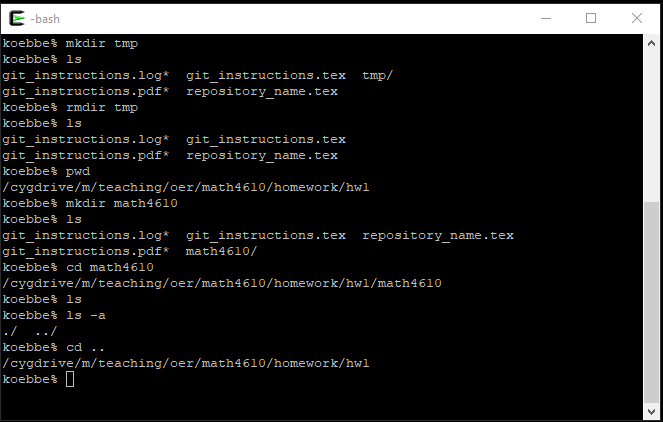
\includegraphics{../images/cygwin_03.png}
\caption{
  Commands for making and removing folders, changing the working directory and
  checking the location of the current folder files and folders. Screenshot
  taken using {\bf Snip \& Sketch}. This is an app on my Windows 10 box}
\end{figure}
\eject
%%%%%%%%%%%%%%%%%%%%%%%%%%%%%%%%%%%%%%%%%%%%%%%%%%%%%%%%%%%%%%%%%%%%%%%%%%%%%%%%
%%%%%%%%%%%%%%%%%%%%%%%%%%%%%%%%%%%%%%%%%%%%%%%%%%%%%%%%%%%%%%%%%%%%%%%%%%%%%%%%
\vskip0.1in\hrule\vskip0.1in
\noindent
{{\bf Cygwin Primer for Math 4610 at USU:} Which Command} 
\vskip0.1in\hrule\vskip0.1in
\noindent
You will want to know what is available for doing work within Cygwin or any
other platform. The which command will let you know if apps or other executables
are available on your version of Cygwin. In particular, it is important to know
if certain compilers (e.g, javac, gcc, f77) are available. A significant number
of tasks you will be asked to complete will require the use of a compiler and
Cygwin has a number of (good) standard compilers for C, C++, and fortran. The
syntax for the command is the following.
\begin{verbatim}

    % which command

\end{verbatim}
\vskip0.1in\hrule\vskip0.1in
\vfill
\begin{figure}[h]
\centering
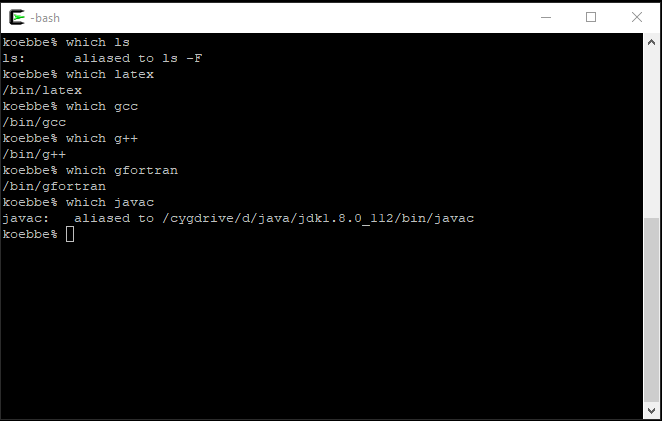
\includegraphics{../images/cygwin_04.png}
\caption{{Screenshot} taken using {\bf Snip \& Sketch}. This is an app on
         my Windows 10 box}
\end{figure}
\eject
%%%%%%%%%%%%%%%%%%%%%%%%%%%%%%%%%%%%%%%%%%%%%%%%%%%%%%%%%%%%%%%%%%%%%%%%%%%%%%%%
%%%%%%%%%%%%%%%%%%%%%%%%%%%%%%%%%%%%%%%%%%%%%%%%%%%%%%%%%%%%%%%%%%%%%%%%%%%%%%%%
\vskip0.1in\hrule\vskip0.1in
\noindent
{{\bf Cygwin Primer for Math 4610 at USU:} A Simple Editing Program} 
\vskip0.1in\hrule\vskip0.1in
\noindent
You will need an editor to create text files. There are a number of editors that
can be downloaded and used in any Cygwin installation. The standard editor that
is always available for linux and unix boxes is \lq vi\rq\. This editor is a bit
rudimentary, but works. Another editor which will be used in by the instructor
in the course is \lq vim\rq. The syntax for starting the editor in a window is
the following.
\begin{verbatim}

    % vim filename

\end{verbatim}
There are a lot of escape sequences it insert text, write a file and so on. If
you are new to vim, you will need to learn at least a few of these editing
commands.
\vskip0.1in\hrule\vskip0.1in
\vfill
\begin{figure}[h]
\centering
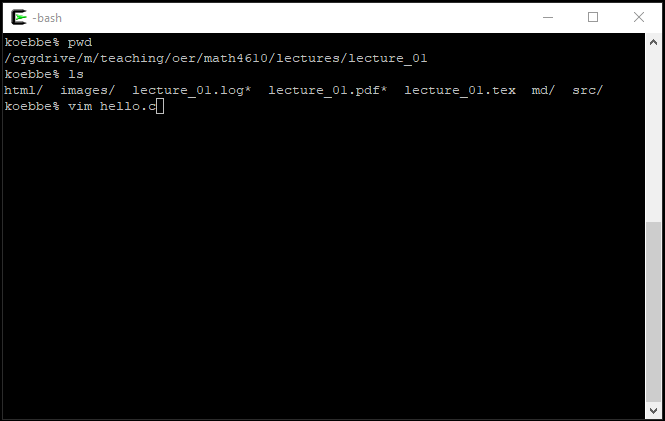
\includegraphics{../images/cygwin_05.png}
\caption{{Screenshot} taken using {\bf Snip \& Sketch}. This is an app on
         my Windows 10 box}
\end{figure}
\eject
%%%%%%%%%%%%%%%%%%%%%%%%%%%%%%%%%%%%%%%%%%%%%%%%%%%%%%%%%%%%%%%%%%%%%%%%%%%%%%%%
%%%%%%%%%%%%%%%%%%%%%%%%%%%%%%%%%%%%%%%%%%%%%%%%%%%%%%%%%%%%%%%%%%%%%%%%%%%%%%%%
\vskip0.1in\hrule\vskip0.1in
\noindent
{{\bf Cygwin Primer for Math 4610 at USU:} First View of the vim Editor} 
\vskip0.1in\hrule\vskip0.1in
\noindent
Below is what the terminal will turn into when you start up the editor on a new
file. To get out of the editor, you can use any of the following commands inside
the editor.
\begin{verbatim}

    :x                  write and exit the editor - saves changes in the file
    :q                  exit the editor if no changes have been made
    :x!                 force a write and exit the editor - saves the file
    :q!                 force an exit of the editor - no changes are saved

\end{verbatim}
Note that there are a few other commands that can be used to save changes. For
example
\begin{verbatim}

    :w                  write and stay in the editor
    :w!                 force a write and stay in the editor

\end{verbatim}
\vskip0.1in\hrule\vskip0.1in
\vfill
\begin{figure}[h]
\centering
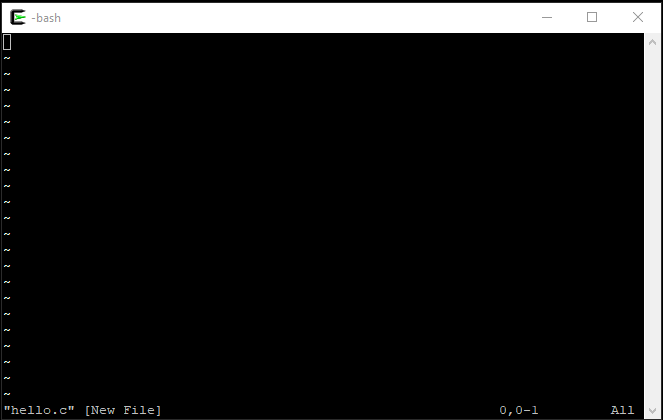
\includegraphics{../images/cygwin_06.png}
\caption{{Screenshot} taken using {\bf Snip \& Sketch}. This is an app on
         my Windows 10 box}
\end{figure}
\eject
%%%%%%%%%%%%%%%%%%%%%%%%%%%%%%%%%%%%%%%%%%%%%%%%%%%%%%%%%%%%%%%%%%%%%%%%%%%%%%%%
%%%%%%%%%%%%%%%%%%%%%%%%%%%%%%%%%%%%%%%%%%%%%%%%%%%%%%%%%%%%%%%%%%%%%%%%%%%%%%%%
\vskip0.1in\hrule\vskip0.1in
\noindent
{{\bf Cygwin Primer for Math 4610 at USU:} An Example of a Text File/Program} 
\vskip0.1in\hrule\vskip0.1in
\noindent
The following screenshot shows a few lines that have been typed into vim that
deinfes a standard hello world example for C. To insert/append characters in the
text file, you can use the following commands to do this. Note that the commands
below do not show up on the screen and the chnages are made where the cursor is
currently located.
\begin{verbatim}

    a                     append text at this point in the file
    o                     open a line after the current line
    O                     open a line before the current line

\end{verbatim}
To end adding or inserting text, use the escape character. Again, the commands
will not show up on screen. Learning everything about vi or vim is a time
consuming process. It is one of those things that you figure out as you go.
\vskip0.1in\hrule\vskip0.1in
\vfill
\begin{figure}[h]
\centering
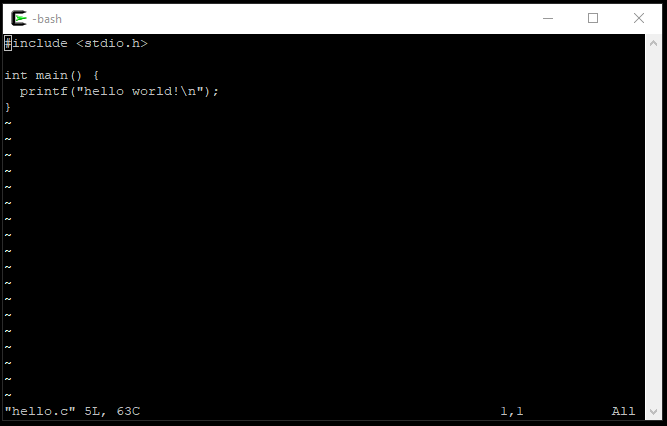
\includegraphics{../images/cygwin_07.png}
\caption{{Screenshot} taken using {\bf Snip \& Sketch}. This is an app on
         my Windows 10 box}
\end{figure}
\eject
%%%%%%%%%%%%%%%%%%%%%%%%%%%%%%%%%%%%%%%%%%%%%%%%%%%%%%%%%%%%%%%%%%%%%%%%%%%%%%%%
%%%%%%%%%%%%%%%%%%%%%%%%%%%%%%%%%%%%%%%%%%%%%%%%%%%%%%%%%%%%%%%%%%%%%%%%%%%%%%%%
\vskip0.1in\hrule\vskip0.1in
\noindent
{{\bf Cygwin Primer for Math 4610 at USU:} Compiling a Program} 
\vskip0.1in\hrule\vskip0.1in
\noindent
Compiling a program is relatively easy at this point in time. To compile the
program on the previous page you should type in
\begin{verbatim}

    % gcc hello.c

\end{verbatim}
The result is an exeutable as seen below. If you want to name the executable
something besides \lq a\rq\ then type the following.
\begin{verbatim}

    % gcc -o hello hello.c

\end{verbatim}
\vskip0.1in\hrule\vskip0.1in
\vfill
\begin{figure}[h]
\centering
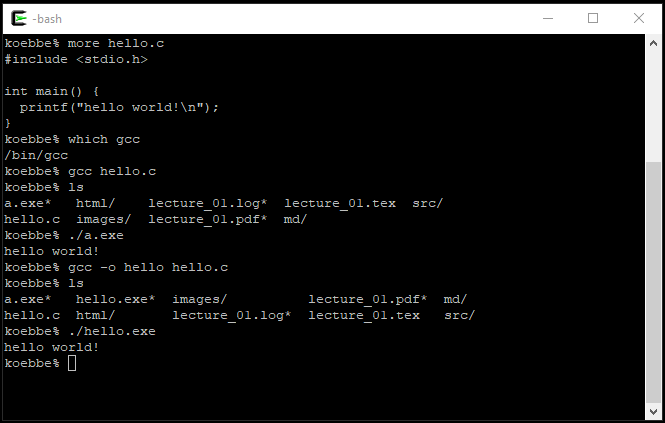
\includegraphics{../images/cygwin_08.png}
\caption{{Screenshot} taken using {\bf Snip \& Sketch}. This is an app on
         my Windows 10 box}
\end{figure}
\eject
%%%%%%%%%%%%%%%%%%%%%%%%%%%%%%%%%%%%%%%%%%%%%%%%%%%%%%%%%%%%%%%%%%%%%%%%%%%%%%%%
%%%%%%%%%%%%%%%%%%%%%%%%%%%%%%%%%%%%%%%%%%%%%%%%%%%%%%%%%%%%%%%%%%%%%%%%%%%%%%%%
\vskip0.1in\hrule\vskip0.1in
\noindent
{{\bf Cygwin Primer for Math 4610 at USU:} Keeping Track of Working Code}
\vskip0.1in\hrule\vskip0.1in
\noindent
It is a good idea to organize your work within assignments and projects. There
is a standard set of folders/directories in linux and unix that most have
adopted. Your instructor follows this idea and usually creates a list of
folders including /src, /data, /bin, and /doc. When computer literate folks see
these folders, they know what is stored in the folders. As an example,
\begin{verbatim}

    % mkdir src
    % mkdir bin

\end{verbatim}
can be used and then the executable the text file can be put into /src and the
binary can be copied into /bin. 
\vskip0.1in\hrule\vskip0.1in
\vfill
\begin{figure}[h]
\centering
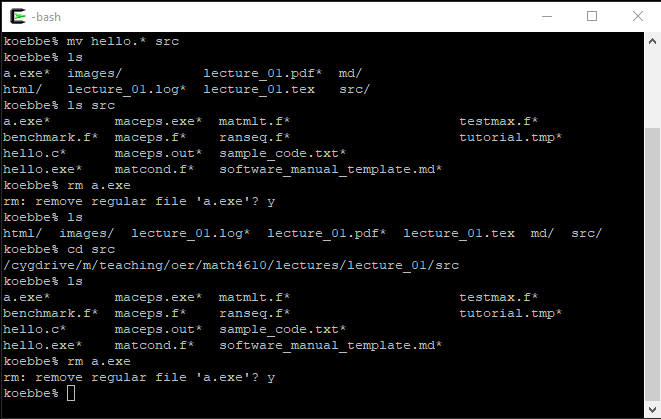
\includegraphics{../images/cygwin_09.png}
\caption{{Screenshot} taken using {\bf Snip \& Sketch}. This is an app on
         my Windows 10 box}
\end{figure}
\eject
%%%%%%%%%%%%%%%%%%%%%%%%%%%%%%%%%%%%%%%%%%%%%%%%%%%%%%%%%%%%%%%%%%%%%%%%%%%%%%%%
%%%%%%%%%%%%%%%%%%%%%%%%%%%%%%%%%%%%%%%%%%%%%%%%%%%%%%%%%%%%%%%%%%%%%%%%%%%%%%%%
\end{document}
